\documentclass{article} % For LaTeX2e
\usepackage{iclr2026_conference,times}

% Optional math commands from https://github.com/goodfeli/dlbook_notation.
\input{math_commands.tex}

\usepackage{hyperref}
\usepackage{url}
\usepackage{graphicx}
\usepackage{booktabs}

\title{Diagnosis Without Execution:\\
Causal-Graph Cases for Multi-Turn Debugging Agents}

% Authors must not appear in the submitted version. They should be hidden
% as long as the \iclrfinalcopy macro remains commented out below.
% Non-anonymous submissions will be rejected without review.

% While \iclrfinalcopy is commented out, iclr2026_conference.sty ignores
% this block and prints "Anonymous authors / Paper under double-blind
% review" itself. FILL IN REAL NAMES before enabling \iclrfinalcopy for
% the camera-ready, or the byline will literally read "Anonymous authors".
\author{Author Name \thanks{Affiliation}\\
Affiliation\\
\texttt{email@example.com}}

%\iclrfinalcopy % Uncomment for camera-ready version, but NOT for submission.
\begin{document}

\maketitle

\begin{abstract}
An agent that debugs \emph{with a person} must elicit the evidence a fix
depends on, avoid the attempts already known to fail, and ground its
conclusion in what the user actually reported. Existing multi-turn
benchmarks measure none of this directly: they either require a
reproducible execution environment---which excludes precisely the
environment-bound problems users bring---or script the user with a
prompt and hope it stays faithful. We annotate 229 resolved public
support threads as causal graphs whose nodes are (system-state,
information-state) pairs and whose edges are clarifications, solutions,
and the attempts each thread itself falsified. The same graph constrains
the simulated user, grounds an execution-free judge, and yields metrics
that need no rubric. Four frontier models separate into two tiers
0.32--0.35 apart; the split survives a judge from a different model
family and reproduces on judge-free counts, while the ordering
\emph{within} a tier does not survive either. Two findings are less
comfortable. Scripted agents bracket the scale, and the weaker pair
scores \emph{below} an agent that asks no questions at all. And swapping
one authored answer for a plausible alternative stops the strongest model
closing the case at all 72\% of the time---it does not adapt, it derails. A third finding is aimed at benchmark builders: handing our
simulator the resolved thread produces detectably leaked turns and yet
moves the mean grade by less than 0.022, so an aggregate score cannot
certify a user simulator. We audit our own instrument in the same
spirit---two harness defects were being scored as model behaviour, two
ablations reversed at full corpus, and one rubric turns out to reward
saying nothing.
\end{abstract}

\section{Introduction}

Debugging with a user is an elicitation problem before it is a repair
problem. The information a fix depends on is usually not in the report:
in our corpus 79\% of the facts a resolution turns on had to be asked
for or measured. An agent that proposes early proposes blind.

Benchmarks for multi-turn software agents take one of two routes, and
both lose the thing we want to measure. Execution-grounded suites
\citep{swebench2024} need a containerised reproduction, which
systematically excludes the environment-bound faults real users
report---drivers, devices, OS integration, account state. Simulated-user
suites \citep{taubench2024,cab2025} avoid that cost by scripting the
user, which moves the problem rather than solving it: a simulator that
has seen the resolution can hand it over, and---as we show in
Section~\ref{sec:leak}---the aggregate score does not move when it does.
A suite therefore cannot tell from its own numbers whether its user is
faithful.

We take a third route. Each case is a resolved public thread annotated as
a causal graph: nodes are (system-state, information-state) pairs, edges
are clarifications the user can answer, solutions with required elements,
and attempts this thread tried and falsified. The graph is an answer key,
not a transcript to replay. The same object then does three jobs: it
bounds what the simulated user may say (it speaks only from its current
node), it gives an execution-free judge something to score against, and
it makes several metrics mechanical---read off the transcript against
the graph rather than scored by a rubric.

Our contributions:

\begin{enumerate}
\item A DSL and a corpus: 229 released cases over 78 repositories, each
      machine-validated and passed by a two-stage model review, with the
      falsified attempts annotated as first-class structure.
\item An evaluation protocol whose central comparison does not depend on
      an LLM judge, and a measurement of what the judge adds where it is
      used.
\item Results on four frontier models, including a counterfactual
      intervention study that the corpus design uniquely enables.
\item Evidence that an aggregate score cannot validate a user simulator:
      a simulator that leaks detectably still scores within 0.022 of a
      clean one. This is a constraint on how any simulated-user benchmark
      can argue for its own fidelity, ours included.
\item An audit of the harness itself. We report the defects we found in
      our own instrument and what each was worth---several would have
      been read as model behaviour---together with two ablations of ours
      whose conclusions reversed when the sample grew.
\end{enumerate}

\section{Related Work}
\label{sec:related}

Table~\ref{tab:related} in the appendix places the neighbours on four
axes---real threads, no execution, a structured oracle, and annotated
falsified attempts. Each holds some; the combination is unoccupied, and
the fourth is the one nothing else has.

\textbf{Execution-grounded agent benchmarks.} SWE-bench
\citep{swebench2024} and its descendants score a patch against a test
suite. This is decisive where it applies and inapplicable where
reproduction is the hard part. CAB \citep{cab2025} builds multi-turn
cases from real GitHub issues but keeps Docker execution, and its own
limitations section reports the resulting selection bias toward
actively-maintained modern repositories. That the cost is affordable is
itself evidence: forbidding execution outright costs a commercial agent
only 1.25 points of resolve rate \citep{torun2026}, and execution-free
critics predict build status at 82\% \citep{llmcritics2025,swejudge2025}.
We give up execution deliberately, and buy back the environment-bound
faults it excludes.

\textbf{Simulated-user benchmarks.} The $\tau$-family
\citep{taubench2024,tau2bench2025}, CAB \citep{cab2025}, and
dialogue-form SWE suites \citep{dialogueswe2026,cirrusbench2026} place an
LLM in the user's seat. Fidelity is the open question, and the field's
own audits are unflattering: $\tau^2$ found its simulator violating its
instructions in 22\% of one domain's dialogues \citep{tau2bench2025}, and
swapping simulators moves measured success by up to 9 points
\citep{lostinsimulation2026}. A simulator conditioned on the resolution
can leak it, and we show in Section~\ref{sec:leak} that such a leak is
invisible in aggregate scores---so a suite cannot certify its own
simulator by observing that its numbers look sensible. We constrain the
simulator with the graph rather than with a prompt, and screen for leaks
directly.

\textbf{Graph- and state-structured evaluation.} Fault trees
\citep{jfta2026} and incident graphs \citep{excytin2026} also score
progress through structure rather than through a final artifact. Their
structures are predefined domain knowledge or recorded logs; ours is
extracted per-case from the thread that resolved it, and carries the
attempts that thread \emph{falsified} as first-class edges---which is
what makes a counterfactual intervention well-posed.

\textbf{Clarification and elicitation.} A line of work scores whether a
model asks a question at all, or resolves a stated ambiguity
\citep{in3_2024,ambigswe2026,userbench2025,multichallenge2025};
multi-turn degradation is well documented \citep{lostinconversation2025}.
We score something narrower and checkable: whether the agent obtained the
specific evidence its own proposal required, at the moment it proposed.

\section{Task Formulation}
\label{sec:task}

\begin{figure}[t]
\centering
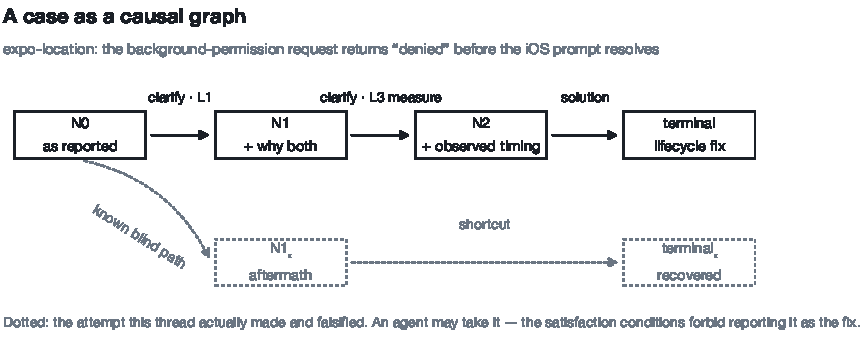
\includegraphics[width=\textwidth]{figures/f1_worked_case.pdf}
\caption{One case as a causal graph. Solid: the diagnostic path. Dotted:
the attempt this thread actually made and falsified, together with the
aftermath state it leads to. An agent may take the falsified branch---the
case's satisfaction conditions forbid \emph{reporting} it as the fix.}
\label{fig:case}
\end{figure}

Figure~\ref{fig:case} shows a complete case. A case is a directed
graph over states. A state pairs a system state with
an information state: what is true of the system, and what has been
established in the conversation. Edges are of three kinds.
\emph{Clarification} edges carry one or more facts the user can supply,
each labelled by how hard it is to obtain: \textbf{L1} any user states it
unprompted, \textbf{L2} inferable from evidence already surfaced,
\textbf{L3} must be asked for or measured. \emph{Solution} edges carry an
intent, a concrete example, and the elements a reply must contain to
count as that fix, plus the information the fix depends on.
\emph{Known-blind} edges are solutions the thread tried and falsified;
they lead to aftermath states from which the investigation continues.

Two derived layers are generated rather than authored: rollback edges out
of every aftermath state, and shortcut copies of a solution edge planted
at earlier states that share its system state, which let an agent skip
evidence---and let the judge grade the skip.

\textbf{The answer-key principle.} The out-edges of a state are what
\emph{could} happen there, not a replay of what the historical
participants did. This is what makes a counterfactual intervention
meaningful (Section~\ref{sec:cf}).

\section{Corpus}
\label{sec:corpus}

The corpus (Figure~\ref{fig:corpus}, Appendix) holds 229 released cases across 78
repositories, the largest contributing 4.8\%, drawn from Mozilla
Bugzilla, PostgreSQL, and permissive-license GitHub repositories, threads
created 2021--2026 (median 37 messages). Per-case structure and the full
breakdown are in Appendix~\ref{app:corpus}. Cases are drafted by a model
from the thread and gated by schema validators and structural lints; a
two-stage review then files findings and independently verifies them.
Single-pass review refuses roughly 95\% of cases, mostly on claims its
own evidence does not support; verification is what makes model review
usable as a release gate. Of 29 cases blocked in the first round, 25
passed after redrafting under hardened rules---their defects came from
the generation prompt, not from the threads.

\textbf{Not recall-solvable.} Handed the opening report alone, with no
opportunity to ask anything, a model names both mechanism and fix class
in 2.2\% of cases (partial credit in a further 3.5\%), with no gradient
by issue year---against 28.8\% for the same model allowed to converse
(Figure~\ref{fig:interaction}). The benchmark measures interactive diagnosis, not
memorisation.

\section{Evaluation Protocol}
\label{sec:protocol}

\textbf{The simulated user} speaks only from its current graph position:
that state's visible symptoms, authored answers to clarifications the
agent actually asked, and---when a stall-insurance mechanism fires---a
reveal that is recorded as such. It is never shown the resolution.

\textbf{Execution-free describes the scoring, not the agent.} What this
benchmark gives up is the \emph{reproduction environment}: there is no
container to rebuild and no test suite to run, because the graph is the
oracle. That is a property of how a transcript is scored, and it places
no requirement on the system being scored. Whatever the agent can
do---search, retrieve, open a sandbox, run an experiment of its own
devising---is part of the capability under measurement, and the harness
neither grants nor withholds it: an adapter receives the leak-free
transcript and returns a turn, and what happens in between belongs to
the agent.

\textbf{What we actually ran} is therefore a baseline rather than the
benchmark's scope: a plain conversational model with no tools, told that
the user is the one executing actions (an accurate statement of that
adapter's situation, which also stops it reporting results it never
obtained). Four toolless rows establish the floor and isolate elicitation
from tooling. They do not characterise tool-using assistants, and we
report no such claim. The release ships a second adapter that drives an
external agent process---one invocation per turn, restoring its own
session---so a sandboxed, retrieving or tool-using system can be measured
by naming it in a command template; we provide the mechanism and no
results under it.

\textbf{Matching.} Each agent turn is read for both acts. A question is
matched against the case's clarifications; a proposal against the current
state's solution edges, producing a \emph{solution call} that records
which required information the agent held at that moment, by level.

\textbf{Metrics.} Case outcomes (\texttt{terminal\_resolved}, forced
walk, ran out), turns, forced reveals per case, and premature proposals
per case are read off the transcript against the graph rather than scored by a rubric. They are not model-free: the matcher deciding whether a turn asks, proposes or both, and which out-edge it hits, is itself an LLM call (Section~\ref{sec:matcherdep}). On top of these, four
LLM rubrics---asks for evidence before proposing, stays inside the
evidence, accounts for the fault, recovers from a failed step---combine
with the graph-supplied grounding rate into a single \texttt{grade}.

\textbf{Cost.} A full row is 229 cases at a median of 20 agent turns, and
the agent call dominates: median latency 105\,s per turn, 117--257
agent-hours per row depending on the model. The four-row main table cost
about 650 agent-hours of wall time, run six cases at a time. Token counts
are not available---the gateway we measured through returns none---so we
report latency, which is what a replicator will actually queue for.

\textbf{Ruling on a difference.} Per-case grades are paired across arms.
A difference is called real only when $|t| > 2.6$ \emph{and} a two-sided
sign test gives $p < 0.01$. This replaced an earlier rule of ``at least
twice the run-to-run drift'', which ignores sample size and consequently
misruled in both directions.

\section{Experiments}
\label{sec:exp}

\begin{table}[t]
\caption{Four models over the released corpus, 30 turns, bracketed by two
scripted agents that read the graph directly (Section~\ref{sec:validity}).
The lower tier sits below the agent that asks nothing. GLM-5.1 is
$n=227$: two cases died on repeated upstream gateway timeouts and are
excluded rather than scored (see Section~\ref{sec:audit}).}
\label{tab:main}
\centering
\begin{tabular}{lrrrrrr}
\toprule
model & grade & resolved & forced walk & ran out & turns & reveals/case \\
\midrule
\emph{conservative} (asks all) & \emph{0.813} & 210 (92\%) & 5 (2\%) & 0 (0\%) & 8 & 0.0 \\
\midrule
gpt-5.6  & \textbf{0.624} & 66 (29\%) & 110 (48\%) & 45 (20\%) & 21 & 3.1 \\
gpt-5.5  & \textbf{0.574} & 71 (31\%) & 103 (45\%) & 47 (21\%) & 20 & 2.8 \\
GLM-5.1  & \textbf{0.306} & 59 (26\%) & 115 (51\%) & 49 (22\%) & 22 & 3.7 \\
Kimi-2.5 & \textbf{0.279} & 52 (23\%) & 103 (45\%) & 70 (31\%) & 21 & 4.0 \\
\midrule
\emph{blind} (asks none) & \emph{0.426} & 169 (74\%) & 47 (21\%) & 6 (3\%) & 6 & 0.9 \\
\bottomrule
\end{tabular}
\end{table}

Table~\ref{tab:main} gives the main result and
Figure~\ref{fig:outcomes} its outcome composition. Two tiers separate by
0.32--0.35 ($t = 32$); within the stronger tier gpt-5.6 leads gpt-5.5 by
0.050 ($t = 5.3$), and between GLM-5.1 and Kimi-2.5 there is nothing to
call. Both within-tier readings are judge-dependent and we do not claim
them---see Section~\ref{sec:judgeswap}. Fewer than a third of cases end in a fix the agent earned, and
roughly half reach a terminal state only because the insurance walked
them there.

\subsection{Where the weaker tier loses}

Figure~\ref{fig:rubrics} (Appendix) localises the gap. It is not confined to any one
rubric, and the largest is \emph{staying inside the evidence}: the GPT
pair scores 0.64--0.71, the other two 0.05--0.09---asserting what their
conversations do not support in nearly every case.

\subsection{The central comparison does not need the judge}

The tier result would be weak if it existed only inside an LLM judge, so
we ask whether it survives with the judge removed entirely. Two per-case
quantities need no rubric to compute: forced reveals, and \emph{premature
proposals}---replies matched as a solution while the conversation sits at
a state whose graph offers no solution edge, meaning the agent proposed a
fix from a position where the case affords none. Both are functions of a
transcript and the graph alone.

\begin{table}[h]
\caption{Premature proposals per case: no judge and no rubric, though the
matcher underneath is still a model (Section~\ref{sec:matcherdep}). The
partition is the one Table~\ref{tab:main} reports.}
\label{tab:judgefree}
\centering
\small
\begin{tabular}{lr@{\hskip 2.5em}lrrl}
\toprule
model & per case & comparison & difference & $t$ & ruling \\
\midrule
gpt-5.6  & 2.36 & gpt-5.6 $<$ Kimi-2.5 & $+1.64$ & $6.95$ & real \\
gpt-5.5  & 2.22 & gpt-5.6 $<$ GLM-5.1  & $+1.44$ & $6.89$ & real \\
GLM-5.1  & 3.79 & gpt-5.5 $<$ GLM-5.1  & $+1.57$ & $7.40$ & real \\
Kimi-2.5 & 4.00 & gpt-5.6 $<$ gpt-5.5  & $-0.14$ & $-0.82$ & not called \\
         &      & GLM-5.1 $<$ Kimi-2.5 & $+0.19$ & $0.83$ & not called \\
\bottomrule
\end{tabular}
\end{table}

Table~\ref{tab:judgefree} gives the result. All three cross-tier
comparisons separate; neither within-tier comparison does. That is the
partition the graded results produce and the partition the swapped judge
produces, arrived at here by counting rather than scoring. The weaker
pair proposes a fix from a state that affords none about 1.6 times more
often per case, which is the behaviour the tier gap is made of.

\subsection{What this removes, and what it does not}
\label{sec:matcherdep}

It removes the judge, not every model. Whether a turn asks or proposes,
and which out-edge it hits, is decided by an LLM matcher; the counts
above are mechanical given those decisions, not given the raw text. The
release also carries a deterministic keyword-and-overlap matcher used as
an offline fallback, and re-deriving this table with it does \emph{not}
reproduce the partition---it marks roughly four times as many proposals
premature and reorders the models. We read that as a fact about the
fallback, which was written as a network-free stand-in rather than a
validated alternative; but it means we cannot claim this result is
independent of the matcher. What we can say is that two judges from
different families agree, and that both read turns segmented by the same
matcher. Establishing the tier result under a competent model-free
matcher is future work, and we would rather name the shared dependency
than let ``no judge'' be read as ``no model''.

\subsection{What the numbers mean: a ceiling and a floor}
\label{sec:validity}

A grade of 0.62 is uninterpretable without knowing what is achievable. We
therefore run scripted agents whose behaviour is fixed by construction
and read against the graph, not against a model. \emph{Conservative}
walks the canonical path and asks every clarification before proposing;
\emph{blind} never asks anything---it burns the edges this thread already
falsified, then guesses down the solutions. Both are deterministic, and Table~\ref{tab:main} brackets the model rows
with them.

Two things follow. First the metrics behave as designed: the profile that
asks everything grounds at 0.989 and proposes prematurely 0.004 times per
case, the profile that asks nothing grounds at 0.358 and proposes
prematurely 0.49 times ($t = -24.2$ and $8.3$ paired). The scale is
anchored, and gpt-5.6 sits about halfway up it, capturing half the
headroom between asking nothing and asking everything.

Second, and less comfortably for the lower tier: GLM-5.1 and Kimi-2.5
score \emph{below} the never-ask floor, by $0.12$ and $0.15$ with
$|t| > 11$. Failing to elicit does not explain this---the floor also
fails to elicit and does better. What differs is what they do instead:
they propose from unsupported states four times per case and assert what
the conversation does not carry. Confidently proposing without evidence
is worse here than proposing almost nothing.

\subsection{The grade rewards silence}
\label{sec:silence}

The same construction supports a sharper test. \emph{Expert} and
\emph{gambler} take \emph{identical} actions---both skip the asking and
fire the same solutions---and differ in one respect: the expert states
the inference it is relying on, drawn from the case's own annotation, so
the reasoning it displays is correct by construction. Any metric that
claims to reward explanation should separate them, and no other metric
should move.

It does not. Grounding does not move ($+0.005$, $t=0.9$), confirming the
actions are identical. But \emph{explanation} moves $+0.016$ and misses
our threshold ($t=2.4$), while \emph{hallucination} moves $+0.207$
against the expert ($t=13.6$) and \emph{proactiveness} $-0.078$
($t=-7.6$). Stating correct reasoning costs $0.060$ of grade
($t=-11.6$): \textbf{the silent agent outscores the explaining one}.

The cause is the construct, not the judge. \emph{Hallucination} asks what
\emph{this conversation} established, so an inference the agent brings to
it reads as assertion beyond the record even when the case certifies it.
That is the defect we identify for retrieval-augmented agents
(Section~\ref{sec:limits}), reached here with no tools at all: it is not
about citations but about any correct reasoning sourced from outside the
dialogue. We report \emph{explanation} as not validated, and the amended
construct shipped with the release targets this as much as tool use.

\subsection{Counterfactual interventions}
\label{sec:cf}

The corpus authors, for clarifications that mattered, an alternative
answer the reporter could plausibly have given, marked with whether the
right fix changes as a result. Replaying a case with one answer swapped
asks whether the agent is conditioning on what the user said. Drawing 60
interventions only from cases whose baseline run closes unaided gives
Figure~\ref{fig:robust} (left):

Changing one answer stops the agent closing the case at all 72\% of the
time (Figure~\ref{fig:robust}, left). It does not switch to a different fix; it stops converging---and it
derails \emph{more} often when the change was marked as not affecting the
diagnosis. On the 17 cases that stayed on the rails, five of ten
interventions that should have changed the fix did.

\subsection{Does the result survive a different judge?}
\label{sec:judgeswap}

The primary judge is from the same family as one of the models it ranks.
Re-judging all four rows with GLM-5.1 under identical rubric definitions
(Figure~\ref{fig:robust}, right) separates two claims that a single
comparison would have conflated.

The swapped judge disagrees substantially about absolute quality: it
lifts the lower tier by $+0.12$ to $+0.13$ while barely moving the upper
($-0.034$ and $-0.004$), so the tier gap roughly halves. What survives
is the tier structure. All three cross-tier comparisons are significant
under both judges (gpt-5.6 over Kimi-2.5: $+0.345$, $t = 31.7$ primary;
$+0.190$, $t = 17.8$ swapped; gpt-5.5 over GLM-5.1: $+0.269$ and
$+0.134$).

The within-tier orderings are a different matter, and neither is solid
enough to claim. gpt-5.6 over gpt-5.5 is significant under the primary
judge ($+0.050$, $t = 5.3$) and not under the swapped one ($+0.020$,
$t = 2.4$). GLM-5.1 over Kimi-2.5 clears the rule under both
($t = 2.61$ primary, $t = 3.24$ swapped)---but the primary figure passes
a $|t| > 2.6$ threshold by $0.005$, which is a decision-boundary
artefact rather than a finding, and we decline to lean on it. We
therefore claim the two tiers, which no judge in our experiments
disturbs, and decline to rank within them. That a hard threshold on a
continuous statistic can be crossed by five thousandths is a limitation
of the ruling procedure, not evidence about the models.

\subsection{What the measurement is robust to}

\textbf{This section previously claimed that replacing the model playing
the user changes nothing, and that claim is withdrawn.} It rested on
$-0.0007$ at $n=48$. Re-run over the full corpus the same intervention
gives $-0.0251$ ($n=226$, bound $0.021$): swapping the simulator lowers
the grade by about half as much as gpt-5.6 leads gpt-5.5, an effect this
paper reports as real.

The two statistics disagree, and the disagreement is itself the finding.
The paired $t$ clears the threshold ($t = -3.08$) while the sign test does
not ($p = 0.081$), so under our conjunctive rule the comparison is not
called. Looking at the distribution explains why: direction is close to
even (125 cases down, 98 up), but the falls are larger than the rises
($-0.105$ against $+0.076$). Changing the simulator does not shift every
case a little; it damages a minority of cases a lot. A rule that requires
consistency of direction will not register that, which is a limitation of
the rule rather than evidence of no effect.

What survives is a weaker claim we still think is worth making. The
literature reports simulator swaps moving measured success by up to
9 points \citep{lostinsimulation2026}, alongside a self-audit in which a
prompted simulator violated its instructions in 22\% of dialogues
\citep{tau2bench2025}. Ours moves 2.5 points. Enumerating the user's
admissible utterances in the case, rather than describing them to a
prompt, appears to reduce the simulator's influence substantially---but
it does not remove it, and we no longer claim that it does.

Two further interventions remain at $n=48$: raising the turn budget from
20 to 30, and re-running the identical configuration. Both of the arms we
did re-run at full corpus moved when the sample grew---this one from
$-0.001$ to $-0.025$, the leak ablation from $+0.037$ to $-0.011$. We
therefore treat the remaining $n=48$ rows as untested rather than as
nulls, and mark them as such in Figure~\ref{fig:all}.

\subsection{Leakage}
\label{sec:leak}

Handing the simulator the resolved thread---the transcript-conditioned
design---produces leaked turns that a lexical screen detects (3 in 916
against 0 in 913 under our production profile). Run over the full corpus,
that leak has \emph{no measurable effect on the grade}: $-0.0114$
($t = -1.36$, sign $p = 0.64$, $n = 229$), with a 99\% bound of $0.022$.

We ran this at $n=48$ first, where it gave $+0.037$ against a bound of
$0.054$, and expected more data to settle a shortfall of power. It did
not: the effect changed sign rather than growing. We report the reversal
because the earlier number would otherwise stand as a near-miss awaiting
more data.

If the score cannot detect a leak, the defence has to be tested
behaviourally instead. We run a scripted \emph{cheater} that opens with
leading questions fishing for future knowledge---what the fix turned out
to be, what the engineer eventually found---and then behaves exactly like
the never-ask \emph{blind} profile. Under the production simulator the
229 fishing turns matched a real graph edge 7 times (3\%): the simulator
declined to answer what its current node does not license. The cheater
ends up $0.035$ below blind rather than above it, because the fishing
burns turns and buys nothing. That is the guarantee stated as a
behaviour rather than as a property of the prompt.

The negative result is more useful to this paper's argument than the
positive one would have been. A simulator can leak the answer and still
produce scores statistically indistinguishable from a clean one---the
leaked turns are demonstrably there, and the aggregate moves by less than
0.022. It follows that \textbf{an aggregate score cannot validate a user
simulator}. A benchmark whose evidence of fidelity is that its numbers
look reasonable has no evidence, and would not notice contamination of
the kind $\tau^2$ found by direct audit in 22\% of one domain's dialogues
\citep{tau2bench2025}. Leak-safety has to come from somewhere the score
cannot vouch for: a structural guarantee plus a direct screen---which is
the design this paper argues for, and this experiment is why the argument
cannot rest on scores.

\section{Auditing the Instrument}
\label{sec:audit}

\begin{figure}[t]
\centering
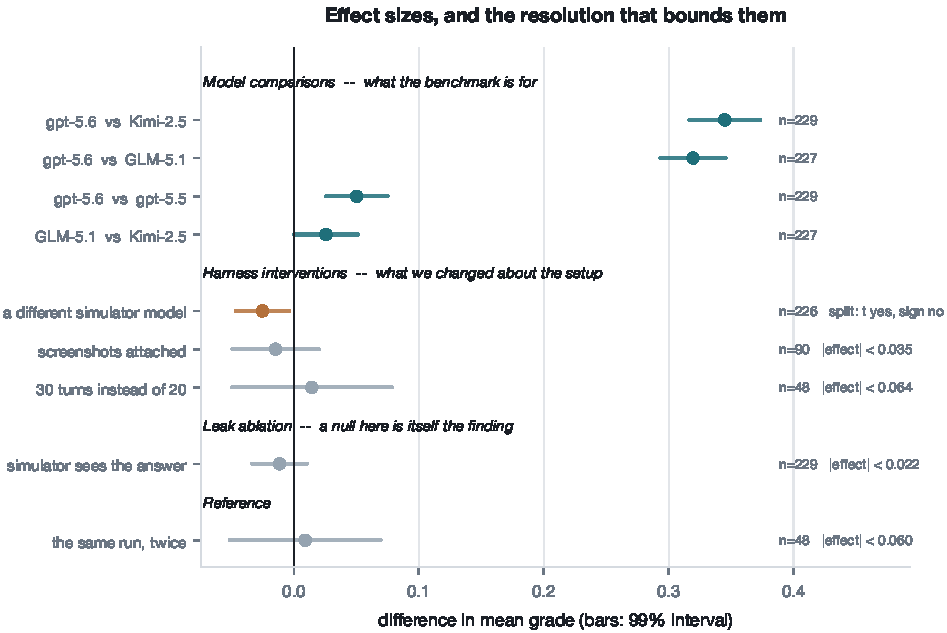
\includegraphics[width=0.86\textwidth]{figures/f6_all_comparisons.pdf}
\caption{Every comparison, with a 99\% interval, grouped by what a null
would mean. Both rows we re-ran at full corpus moved: the
simulator swap from $-0.001$ to $-0.025$ (orange---the paired $t$ clears
our threshold while the sign test does not, so it is not called), and the
leak ablation to $-0.011$, bounding at $0.022$ the grade effect of handing
the simulator the answer, which is why the score cannot detect leakage.
Rows are coloured by the paper's ruling rule rather than by whether the
interval clears zero. Each uncalled row is annotated with the effect it
can exclude; the remaining $n=48$ rows exclude only $\pm0.06$.}
\label{fig:all}
\end{figure}

Figure~\ref{fig:all} places every comparison we ran on one axis, with
the same configuration run twice as the bottom row. Building this
benchmark produced findings about the benchmark. We report
them because several would otherwise have been read as model behaviour.

\textbf{Most intervention events were our fault} (Figure~\ref{fig:defects}).
Before repair, 44\% of
cases in every row triggered a forced reveal at a rate that barely varied
across models---a signal belonging to the harness. Decomposed, only
7--11\% reflected an agent failing a modelled path; the rest were a
matcher that could not represent a turn containing both a question and a
proposal, a simulator that fabricated negative results for fixes the case
never modelled, and a canonical-path search that refused the falsified
edges most threads pass through, killing half of every run at a median of
turn 5.

\textbf{Two published findings were rubric artefacts.} A rubric asking
whether the agent ``proactively gathered info'' scored every model
0.92--0.97 and supported a conclusion that elicitation was saturated.
A judge-independent count contradicted it the whole time---premature
proposals per case run 2.36 to 4.00 across the four models---and under a
rubric that asks whether the evidence was in hand \emph{before} the
proposal, the scores track that count at Spearman $-0.80$. Separately, an
under-specified rubric made two judges score different constructs and
produced an apparent finding that the tier gap belonged to the judge; it
did not survive the rubrics being written down.

\textbf{A harness failure was being scored as model behaviour, in one row
only.} Two cases in the GLM-5.1 row produced zero-turn transcripts after
the upstream gateway timed out, and the judge scored those empty
transcripts $0.0$ rather than skipping them---so an infrastructure
failure entered the table as the model's worst possible performance, and
entered only one of the four rows. The effect is small ($0.303$ against
a clean $0.306$) and its direction is what matters: it is a
row-asymmetric penalty, so every comparison involving that row was
biased by an amount no re-run of the other rows would reveal. We found it
by auditing termination reasons per row rather than by checking that each
row had 229 entries, which it did. The two cases fail reproducibly on the
same upstream timeout across two further attempts, so they are excluded
and the row is reported at $n=227$ rather than repaired. The judge now
has an explicit guard, and our reconciliation checks per-row termination
reasons rather than row totals.

\textbf{Our own $n=48$ ablations were not trustworthy, and we found out
by re-running them.} Two of the harness interventions in this paper were
originally measured on a 48-case variance subset. Re-run over the full
corpus, both moved: the leak ablation from $+0.037$ to $-0.011$, changing
sign, and the simulator swap from $-0.0007$ to $-0.025$, turning what we
had described as a clean null into an effect half the size of a model
difference we report as real. Neither reversal was a change in the
benchmark: the smaller sample was reporting noise inside a bound
($\pm0.06$) loose enough to hold it. A null is a claim about a bound, and
a bound three times wider than the effects under discussion supports no
claim at all; the remaining $n=48$ rows are reported as untested.

\textbf{The grade resolves less than four rubrics suggest.} Over 914
case-rows the rubrics correlate at $|\rho| = 0.58$--$0.74$, so the grade
is nearer one dimension than four; with \emph{explanation} also shown
above not to respond to explaining, a single model's rubric profile is
not four separable competencies. Grade tracks conversation length
($\rho \approx -0.47$), expected but worth stating. Difficulty, though,
is \emph{not} explained by graph size---nodes, edges, L3 clarifications
and known-blind edges each correlate with mean grade at $|\rho| < 0.09$,
and the hardest and easiest quartiles are structurally near-identical
while differing by 0.25 in grade.

\textbf{What we now check on every run.} Ten offline simulator
invariants; a row-integrity reconciliation of transcripts against metrics
against judgments, flagging when the missing cases are disproportionately
successes; a validity gate on empty replies; a leak screen; and a rubric
sanity check against the behavioural counts.

\section{Limitations}
\label{sec:limits}

\textbf{The judge was never validated against a human.} This is the
paper's largest gap. The corpus is machine-drafted and machine-reviewed
with the audit trail published, and the judge is a model; nothing here
establishes that its scores are \emph{right}. Neighbouring work does
better on exactly this axis---CAB reports 65.9\% judge--human agreement
\citep{cab2025}---and we have no comparable number.

We can bound the other side. Re-judging the same transcripts with the
same judge moves the per-case grade by $0.026$ on average ($r=0.97$,
$n=229$; $0.023$, $r=0.98$ on the lower-scoring row, so reliability does
not depend on where a model sits). At $n=229$ that contributes about
$0.002$ to any corpus mean, and it is already inside the paired standard
deviation the $t$-tests use. It also decomposes the per-case instability
reported above: of the $0.10$--$0.12$ drift between identical runs,
$0.026$ is the judge and the rest is the agent's sampling. \emph{Hallucination} is
the least self-consistent rubric ($0.089$, $r=0.84$) and carries our
most-cited rubric reading, which we flag rather than discount. So
reliability is not the problem---validity is, and self-agreement cannot
speak to it: two passes of one model can be wrong together.

\textbf{The instrument has a resolution, and some of our own
interventions sit below it.} No claim here rests on an individual case
(Figure~\ref{fig:reliability}). Aggregated, the 99\% interval is about
$\pm0.025$ at full corpus and $\pm0.06$ on the 48-case subset; the model
comparisons run $5$--$13\times$ the full-corpus floor and are safe. The
harness interventions are not: we re-ran two at full corpus and both
changed conclusion, so the two still on 48 cases are reported as untested
rather than as nulls.

\textbf{A tool-using agent would be scored unfairly.}
Section~\ref{sec:silence} shows the grounding construct penalising correct
reasoning brought from outside the dialogue, measured with no tools at
all; an agent that cites a release note is the same case. The amended
construct---supported by the conversation \emph{or} by a checkable
citation, with an uncheckable one counted worse than an unhedged
guess---ships with the release and is selectable, but we report no
results under it, since scores from two constructs are not comparable and
this paper already had to retract one finding that was that mistake made
across two judges. These results describe elicitation in a
toolless condition and should not be transferred to retrieval-augmented
assistants.

\section{Conclusion and release}

Diagnosing a fault with a person is the work of finding out what is true,
so a benchmark for it must score the finding-out, not the final artifact.
Annotating each thread as a causal graph constrains the simulated user by
structure rather than instruction, makes several metrics mechanical, and
---because the graph records what \emph{could} have happened---makes a
counterfactual intervention well posed. Frontier models split into two
tiers, driven by proposing fixes from positions the case does not
support. The result we would most like other builders to take, though, is
the uncomfortable one: a simulator that leaks detectably still scored
within 0.022 of a clean one, so a suite cannot use its own numbers as
evidence that its user is faithful.

\subsubsection*{Reproducibility Statement}

The benchmark, the 229 released cases, the harness, and every transcript
and judgment file behind the tables here are released together; the
scripts that produce each figure read those files directly, so every
number in this paper can be recomputed from the artifact. Case outcomes,
turn counts, forced reveals and premature proposals are deterministic
turn counts, forced reveals and premature proposals are mechanical functions of a transcript, a graph, and the matcher. Two things are
not reproducible in the strict sense and we would rather name them than
imply otherwise. Model replies are sampled, so a re-run does not
reproduce a transcript; per-case grades drift by 0.10--0.12 in mean
absolute terms across identical runs, which is why every claim here is an
aggregate over the corpus and why the ruling procedure is a paired test.
And the two GPT endpoints we measured expose no snapshot identifier
(Section~\ref{sec:access}), so those rows can be re-run but not pinned to
a fixed model revision.

\subsubsection*{Ethics Statement}

Code is released under Apache-2.0 and the curation layer under CC BY 4.0.
The corpus is built from public bug trackers and issue threads under
permissive terms, and we redistribute thread content rather than
re-hosting private data. Usernames are pseudonymised and the curation
layer is released separately from the thread text so that the annotation
can be reused without the identities. The people who wrote these threads
were reporting bugs, not volunteering for a benchmark; we therefore
restrict the release to sources whose licences permit redistribution,
carry the original attribution, and will honour removal requests for
individual threads. The cases describe software faults and their fixes
and we see no dual-use concern beyond that. Coverage is bounded in ways
worth stating: threads are English-only and from open-source projects, so
the corpus speaks to that population and not to proprietary or
non-English support traffic. The benchmark measures
diagnostic dialogue and should not be read as a safety evaluation: a
model can score well here and still be unsafe to deploy in a support
role.

\subsubsection*{Use of Large Language Models}

LLMs are not an incidental writing aid in this work; they are part of the
instrument, and we describe where. Each case in the corpus was
\emph{drafted} by a model from the source thread and then \emph{reviewed}
by a two-stage model process that files findings and independently
verifies them, with schema validators and structural lints as hard gates.
No case was authored by a human annotator, and the judge that produces
the rubric scores is itself a model. This is the central limitation of
the corpus and is discussed as such rather than buried: we release the 55
drafts that review rejected alongside the 229 that passed, so the review
layer can be audited rather than trusted. The simulated user is likewise
model-driven, constrained by the graph. In preparing the manuscript, an
LLM was used for drafting and editing prose and for writing analysis
code; the experimental design, the decisions about what to claim and what
to withdraw, and the final text are the authors' responsibility.

\bibliography{iclr2026_conference}
\bibliographystyle{iclr2026_conference}

\appendix
\section{Additional audit findings}
\label{app:audit}

\textbf{A stale summary survived the repair.} Dropping those cases did
not update the judgment file's cached aggregate---recomputed only when a
case is judged---so it kept reporting the contaminated mean over a count
it no longer held, and the repair printed that back as the new result.
Our checks now recompute every aggregate from the per-case records and
refuse the file when the two disagree.

\section{Model access and version pinning}
\label{sec:access}

All four systems were reached through a single hosted OpenAI-compatible
gateway, so the comparison is internally consistent: identical harness,
identical prompts, identical judge. Exact versions are only partly
pinnable, and we state which. Two endpoints resolve to reportable model
identifiers (\texttt{kimi-k2.5}; a vendor-hosted GLM-5.1 deployment,
which may differ from the stock release and which we name as
``GLM-5.1'' only for readability). The two GPT endpoints return an
opaque deployment identifier and expose no snapshot string, so we cannot
pin the precise revision behind the ``gpt-5.6'' and ``gpt-5.5'' rows.
Readers should treat the model names as labels for the endpoints we
measured rather than as verifiable version claims, and the released
transcripts---not the model names---as the reproducible artifact.

\begin{table}[t]
\caption{Where this benchmark sits. \emph{Real threads}: cases derived
from support or issue threads rather than synthesised. \emph{No
execution}: scoring needs no reproduction environment. \emph{Structured
oracle}: progress is scored against an explicit state structure rather
than a final artifact or a linear checkpoint list. \emph{Falsified
attempts}: the paths the source case tried and ruled out are annotated as
first-class edges.}
\label{tab:related}
\centering
\footnotesize
\begin{tabular}{lcccc}
\toprule
 & real & no & structured & falsified \\
 & threads & execution & oracle & attempts \\
\midrule
SWE-bench \citep{swebench2024}          & \checkmark & & & \\
CAB \citep{cab2025}                     & \checkmark & & & \\
Dialogue SWE-Bench \citep{dialogueswe2026} & \checkmark & & & \\
CirrusBench \citep{cirrusbench2026}     & \checkmark & & partial & \\
$\tau$/$\tau^2$ \citep{taubench2024,tau2bench2025} & & \checkmark & \checkmark & \\
JFTA-Bench \citep{jfta2026}             & & \checkmark & \checkmark & \\
ExCyTIn \citep{excytin2026}             & \checkmark & \checkmark & \checkmark & \\
\midrule
This work                               & \checkmark & \checkmark & \checkmark & \checkmark \\
\bottomrule
\end{tabular}
\end{table}

\section{Corpus statistics}
\label{app:corpus}

\begin{table}[h]
\caption{Per-case structure of the 229 released graphs. Counts are over
the released corpus and are recomputable from the artifact.}
\label{tab:corpus}
\centering
\begin{tabular}{lrrrr}
\toprule
 & mean & median & max & total \\
\midrule
states (nodes)            & 6.2 & 6 & 10 & 1416 \\
transitions (edges)       & 5.4 & 5 &  9 & 1234 \\
clarifications            & 5.5 & 5 & 18 & 1268 \\
solution edges            & 2.5 & 2 &  7 &  575 \\
known-blind edges         & 0.9 & 1 &  5 &  216 \\
\bottomrule
\end{tabular}
\end{table}

Edges are 659 clarification-only, 555 solution-only, and 20 mixed.
Clarifications carry an obtainability level: 17\% \textbf{L1} (any user
volunteers it), 4\% \textbf{L2} (inferable from what is already on the
table), and 79\% \textbf{L3} (must be asked for or measured)---the
distribution behind the claim that most evidence a resolution depends on
has to be elicited. 147 cases (64\%) contain at least one known-blind
edge, so the falsified-attempt structure is not a rare decoration: it is
present in roughly two thirds of the corpus and is what makes a
counterfactual intervention well posed. The 229 cases come from 78
distinct repositories with the largest contributing 11 cases (4.8\%);
no single project dominates.

\begin{figure}[t]
\centering
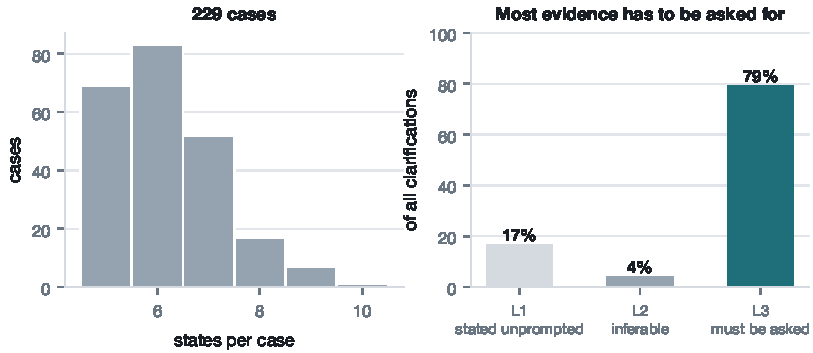
\includegraphics[width=\textwidth]{figures/f8_corpus.pdf}
\caption{Corpus shape. Most evidence a resolution depends on has to be
asked for: 79\% of clarifications are L3.}
\label{fig:corpus}
\end{figure}

\begin{figure}[t]
\centering
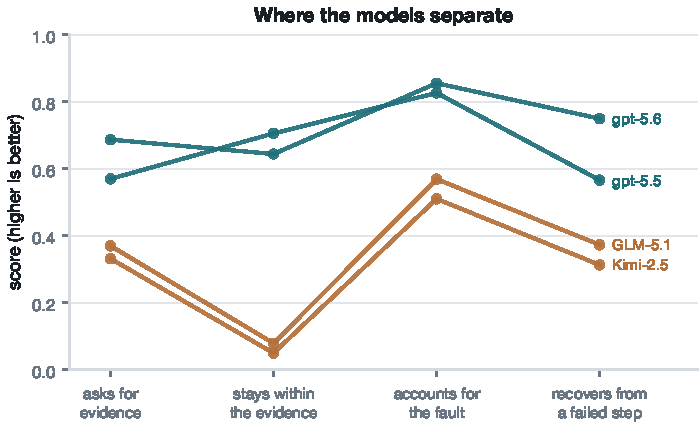
\includegraphics[width=0.86\textwidth]{figures/f2_rubrics.pdf}
\caption{The tiers separate on all four rubrics and never cross. The
deepest gap is staying inside the evidence.}
\label{fig:rubrics}
\end{figure}

\begin{figure}[t]
\centering
\begin{minipage}[t]{0.48\textwidth}
\centering
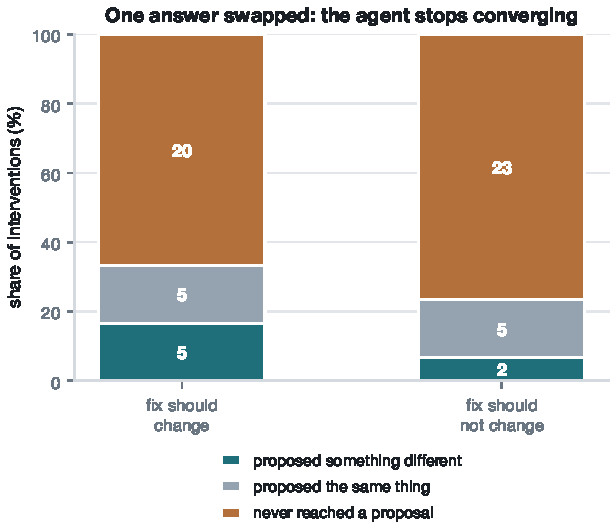
\includegraphics[width=\textwidth]{figures/f9_counterfactual.pdf}
\end{minipage}\hfill
\begin{minipage}[t]{0.48\textwidth}
\centering
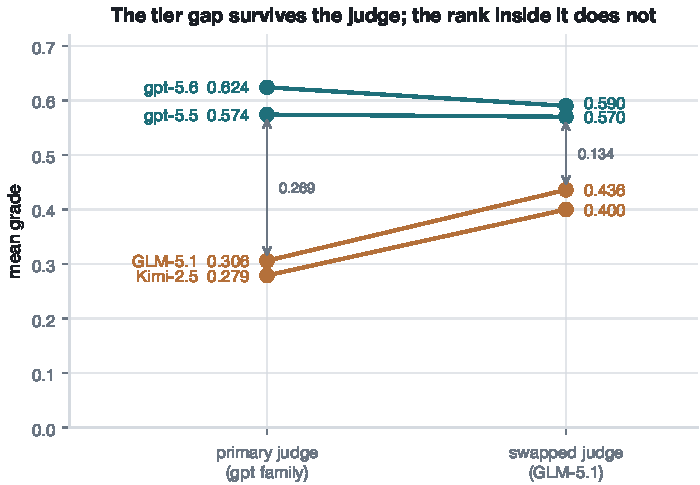
\includegraphics[width=\textwidth]{figures/f10_judge_swap.pdf}
\end{minipage}
\caption{Left: swapping one authored answer does not redirect the agent,
it stops it---and the collapse is worse in the column where the
diagnosis was \emph{not} supposed to move. Right: all four rows under two
judges, same transcripts, same written rubrics. They disagree
substantially about absolute quality; the tier separation survives both
and the ordering within a tier does not.}
\label{fig:robust}
\end{figure}

\section{Supporting figures}

These four figures support claims made in the main text and are
placed here for space.

\begin{figure}[t]
\centering
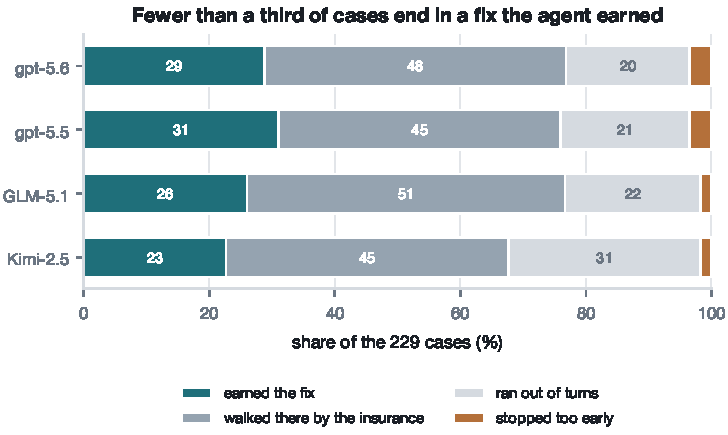
\includegraphics[width=0.82\textwidth]{figures/f3_outcomes.pdf}
\caption{How cases end. The tiers differ less in fixes earned than in
what happens when they fail: Kimi-2.5 exhausts its turn budget on 31\%
of cases against gpt-5.6's 20\%, while roughly half of every row reaches
a terminal state only because the stall insurance walked it there.}
\label{fig:outcomes}
\end{figure}

\begin{figure}[t]
\centering
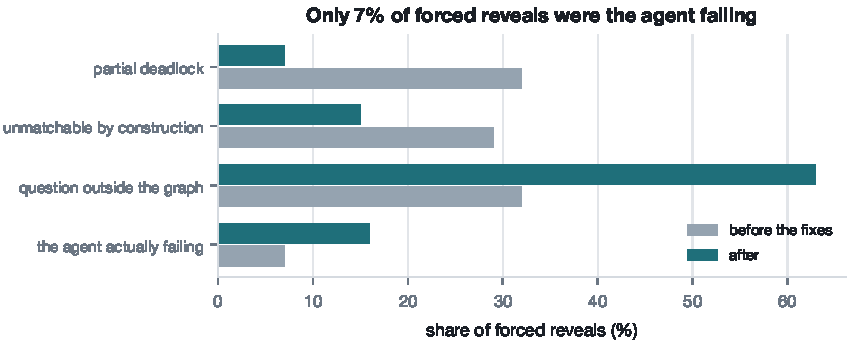
\includegraphics[width=0.66\textwidth]{figures/f4_harness_defects.pdf}
\caption{Decomposing the benchmark's own intervention events before
repair. Read as a model metric this looked like agents stalling on half
of all cases; almost all of it was the instrument.}
\label{fig:defects}
\end{figure}

\begin{figure}[t]
\centering
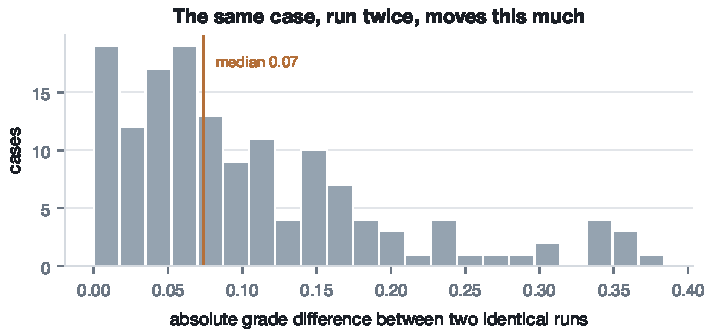
\includegraphics[width=0.58\textwidth]{figures/f5_reliability.pdf}
\caption{The same configuration run twice. Per-case grades move enough
that no claim in this paper rests on an individual case; aggregate
differences of the size we report survive it, and this is why the ruling
procedure is a paired test rather than a threshold on the difference.}
\label{fig:reliability}
\end{figure}

\begin{figure}[t]
\centering
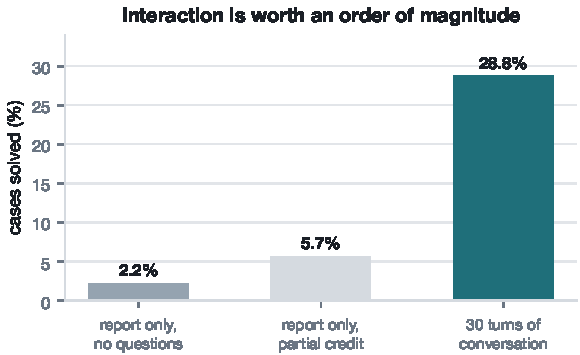
\includegraphics[width=0.52\textwidth]{figures/f7_interaction_value.pdf}
\caption{The same model on the same cases, with and without the ability
to ask. Given the opening report alone it names mechanism and fix class
in 2.2\% of cases; given the conversation, 28.8\%. The benchmark is
measuring elicitation, not recall.}
\label{fig:interaction}
\end{figure}


\end{document}
